\documentclass[11pt,a4paper]{article}

% Packages
\usepackage[utf8]{inputenc}
\usepackage[spanish, es-tabla]{babel}
\usepackage{caption}
\usepackage{listings}
\usepackage{adjustbox}
\usepackage{enumitem}
\usepackage{boldline}
\usepackage{amssymb, amsmath}
\usepackage[margin=1in]{geometry}
\usepackage{xcolor}
\usepackage{enumerate}
\usepackage{hyperref}
\usepackage{graphics, graphicx, float}
\usepackage{titlesec} %\titleformat

% Meta
\title{Inteligencia de Negocio: Práctica 3
	\\\medskip \large Aplicación Real: Competición en DrivenData}
\author{José Antonio Álvarez Ocete - 77553417Q \\ joseantonioao@correo.ugr.es}
\date{ \today }

% Custom
\providecommand{\abs}[1]{\lvert#1\rvert}
\setlength\parindent{0pt}
\definecolor{Light}{gray}{.90}
\setlength{\parindent}{1.5em} %sangria

% Subsubsubsection (|paragraph)
\setcounter{tocdepth}{4}
\setcounter{secnumdepth}{4}

\begin{document}	
	
	\maketitle 
	\newpage
	\tableofcontents
	\newpage
	
	\section{Introducción}
	
	En esta última práctica participamos en una competición DrivenData - Richter's Predictor: Modeling Earthquake Damage (\url{https://www.drivendata.org/competitions/57/nepal-earthquake/submissions/}). Nuestro objetivo será predecir la severidad de los daños tras un terremoto en Nepal. 

	\section{Intentos realizados}
	
	Presentamos a continuación los intentos realizados para la competición.
	
	\begin{figure}[H] 
		\centering
		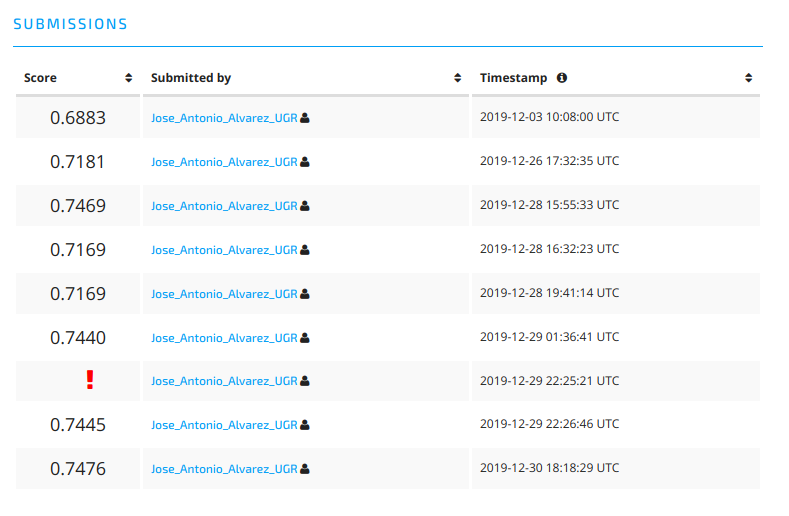
\includegraphics[scale=0.6]{../capturas/submissions}
		\caption{Submissions - resumen de los intentos realizados}
	\end{figure}
	
	
	\subsection{Intento 1: Ejemplo de Jorge}
	
	Primera subida realizada en clase.
	
	\begin{itemize}
		\item \textbf{Fecha y hora}: 2019-12-03 10:08:00 UTC
		\item \textbf{F1-score obtenido}: 0.6883
		\item \textbf{Preprocesado}: \emph{Category to number} aplicado a las variables categóricas.
		\item \textbf{Algorimo empleado}: LGBM
		\item \textbf{Parámetros de los algoritmos}: \emph{objective='regression\_l1', n\_estimators=200, n\_jobs=4}
	\end{itemize}
	
	\begin{figure}[H] 
		\centering
		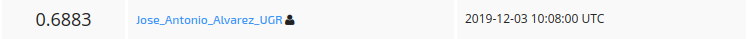
\includegraphics[scale=0.6]{../capturas/T1}
		\caption{Intento 1}
	\end{figure}
	
	
	\subsection{Intento 2: Get Dummies}
	
	Primer día de trabajo. Trasteando un poco el preprocesado sin tocar el algoritmo en si, cambió \emph{Category to number} por \emph{Get Dummies}. Resulta dar unos resultados mucho mejores. Sin embargo, el número de atributos aumenta a mas de seis decenas. Esto tendrá repercusiones posteriormente en el tiempo de ejecución de los algoritmos, lo que acaba siendo un factor decisivo en esta competición. Aún así, ni si quiera se plantéa quitarlos debido a la increible mejora que proporcionan.
	
	\begin{itemize}
		\item \textbf{Fecha y hora}: 2019-12-26 17:32:35 UTC
		\item \textbf{F1-score obtenido}: 0.7181
		\item \textbf{Preprocesado}: \emph{Get Dummies}.
		\item \textbf{Algorimo empleado}: LGBM
		\item \textbf{Parámetros de los algoritmos}: \emph{objective='regression\_l1', n\_estimators=200, n\_jobs=4}
	\end{itemize}
	
	\begin{figure}[H] 
		\centering
		
\includegraphics[scale=0.6]{../capturas/T2}
		\caption{Intento 2}
	\end{figure}
	
	\subsection{Intento 3: Noise reduction, feature selection y XGBoosting}
	
	Sigo trabajando el primer día. Intento reducir ruido utilizando los algoritmos vistos en clase. Tras no conseguir que funcione nada en Python intento trabajar en R. Me dispongo a usarlo pero los algoritmos me dan problemas de dependencias que no se resolver. Deshecho la idea de limpiar ruido con algoritmo conocidos con perspectiva de quizás implementar SMOTE a mano. \\
	
	Comienza el segundo día. Intento aplicar selección de características. Utilizo los algoritmos de Mlxtend. Los algoritmos SFS, SBS, SFFS, SBFS tienen problemas de dependencias (les falta un import!) y no puedo ejecutarlos. Pruebo con ExhaustiveForwardSearch (EFS) pero no acaba, como es natural. Tambien pruebo a estudiar una matriz de correlaciones. Como en principio no acaba de ejecutar utilizo undersampling para ejecutarlo en un subgrupo de las instancias. Tampoco acaba. \\
	
	Tercer día de trabajo. Empiezo a usar SelectKBest (un \emph{wrapper} que selecciona los k mejores atributos). Para ello le vamos dando distintos valores a k y realizamos un estudio con cuál da mejor resultado. Puesto que toma mucho tiempo de ejecución, mientras tantoconfiguro el algoritmo XGBoosting, ya que mis ataques al preprocesado no han tenido absolutamente ningún resultado. \\
	
	Subimos la ejecución de XGBoosting con asombrosamente buenos resultados. Las conclusiones del SelectKBest se estudian en el siguiente intento. \\
	
	\begin{itemize}
		\item \textbf{Fecha y hora}: 2019-12-28 15:55:33 UTC
		\item \textbf{F1-score obtenido}: 0.7469
		\item \textbf{Preprocesado}: \emph{Get Dummies}.
		\item \textbf{Algorimo empleado}: XGBoosting
		\item \textbf{Parámetros de los algoritmos}: \emph{(n\_estimators=600 reg\_alpha=0.3, seed=123456, eta=0.1, max\_depth=10}
	\end{itemize}
	
	\begin{figure}[H] 
		\centering
		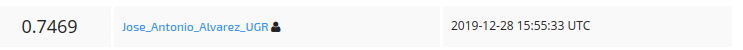
\includegraphics[scale=0.6]{../capturas/T3}
		\caption{Intento 3}
	\end{figure}
	
	\subsection{Intento 4: Estudio de SelectKBest}
	
	Tras completar el estudio de Feature Selection con SelectKBest subo el mejor valor de SelectKBest (k=33) con lgbm. Obtengo 0.7169, peor que el resultado original (T2 - 0.7181) sin preprocesado.
	
	\begin{itemize}
		\item \textbf{Fecha y hora}: 2019-12-28 16:32:23 UTC
		\item \textbf{F1-score obtenido}: 0.7169
		\item \textbf{Preprocesado}: \emph{Get Dummies} y \emph{SelectKBest} con \emph{k=33}.
		\item \textbf{Algorimo empleado}: LGBM
		\item \textbf{Parámetros de los algoritmos}: \emph{objective='regression\_l1', n\_estimators=200, n\_jobs=4}
	\end{itemize}
	
	\begin{figure}[H] 
		\centering
		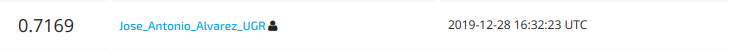
\includegraphics[scale=0.6]{../capturas/T4}
		\caption{Intento 4}
	\end{figure}
	
	\subsection{Intento 5: Subida errónea}
	
	En este intento subí de forma equivocada los resultados del intento 4.
	
	\subsection{Intento 6: SelectKBest con XGBoosting}
	
	Unimos a continuación los resultados de los dos intentos anteriores, combinando la mejor configuración obtenida de XGBoosting con el preprocesado de SelectKBest con k=33. Obtenemos un F1-score de 0.7440, ligeramente peor que el 0.7469 del intento con XGBoosting sin preprocesado pero en la mitad de tiempo. \\
	
	\begin{itemize}
		\item \textbf{Fecha y hora}: 2019-12-29 01:36:41 UTC
		\item \textbf{F1-score obtenido}: 0.7440
		\item \textbf{Preprocesado}: \emph{Get Dummies} y \emph{SelectKBest} con \emph{k=33}.
		\item \textbf{Algorimo empleado}: XGBoosting
		\item \textbf{Parámetros de los algoritmos}: \emph{(n\_estimators=600 reg\_alpha=0.3, seed=123456, eta=0.1, max\_depth=10}
	\end{itemize}
	
	\begin{figure}[H] 
		\centering
		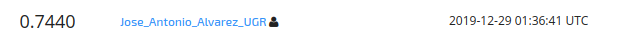
\includegraphics[scale=0.6]{../capturas/T6}
		\caption{Intento 6}
	\end{figure}
	
	\subsection{Intentos 7 y 8: Selección de instancias y salto a stacking}
		
	En esta etapa final de la competición comenté mis resultados con mis compañeros. Dado que ha ellos les estaba yendo bien con la técnica de Stacking me propuse a usarla combinándola con el preprocesado que había estado usando hasta ahora. Si bien se ha demostrado en dos ocasiones que este preprocesado reduce la calidad del predictor obtenido a posteriori, si que reduce significativamente el tiempo de ejecución. Utilizo por tanto el preprocesado buscando lanzar algoritmos mucho más pesados. \\
	
	Me temo que por alguna razón que desconozco no tengo guardados los parámetros de la subida número 7, pero ambas son exactamente iguales: aplicación de stacking con preprocesado de SelectKBest, aumentando los valores de los parámetros del 7 al 8. La última subida llevo un tiempo de ejecución de entre 10 y 17 horas (lo dejé por la noche ejecutando) y dado el día que era y que la alternativa que me quedaba era ejecutar stacking con mayores valores de los parámetros (añadir otros estimadores tampoco me daba mejores resultados), di por terminada la competición. A día 7 de enero estoy en la posición 88 con un F1-score final de 0.7476.
	
	\begin{itemize}
		\item \textbf{Fecha y hora}: 2019-12-29 22:26:46 UTC y 2019-12-30 18:18:29 UTC.
		\item \textbf{F1-score obtenido}: 0.7445 y 0.7476.
		\item \textbf{Preprocesado}: \emph{Get Dummies} y \emph{SelectKBest} con \emph{k=33}.
		\item \textbf{Algorimo empleado}: Stacking con estimadores RandomForest y XGBoosting.
		\item \textbf{Parámetros de los algoritmos}: XGBoosting: \emph{(n\_estimators=600, seed=323232, eta=0.1, max\_depth=10}. RandomForest: \emph{n\_estimators=200, n\_jobs=-1, max\_depth=50, warm\_start="True"}
	\end{itemize}
	
	\begin{figure}[H] 
		\centering
		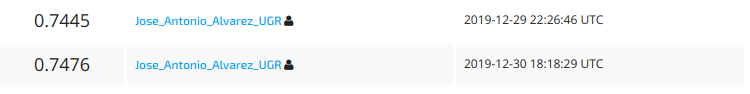
\includegraphics[scale=0.6]{../capturas/T78}
		\caption{Intento 7 y 8}
	\end{figure}
		
	
\end{document}